% Options for packages loaded elsewhere
\PassOptionsToPackage{unicode}{hyperref}
\PassOptionsToPackage{hyphens}{url}
%
\documentclass[
]{book}
\usepackage{amsmath,amssymb}
\usepackage{lmodern}
\usepackage{iftex}
\ifPDFTeX
  \usepackage[T1]{fontenc}
  \usepackage[utf8]{inputenc}
  \usepackage{textcomp} % provide euro and other symbols
\else % if luatex or xetex
  \usepackage{unicode-math}
  \defaultfontfeatures{Scale=MatchLowercase}
  \defaultfontfeatures[\rmfamily]{Ligatures=TeX,Scale=1}
\fi
% Use upquote if available, for straight quotes in verbatim environments
\IfFileExists{upquote.sty}{\usepackage{upquote}}{}
\IfFileExists{microtype.sty}{% use microtype if available
  \usepackage[]{microtype}
  \UseMicrotypeSet[protrusion]{basicmath} % disable protrusion for tt fonts
}{}
\makeatletter
\@ifundefined{KOMAClassName}{% if non-KOMA class
  \IfFileExists{parskip.sty}{%
    \usepackage{parskip}
  }{% else
    \setlength{\parindent}{0pt}
    \setlength{\parskip}{6pt plus 2pt minus 1pt}}
}{% if KOMA class
  \KOMAoptions{parskip=half}}
\makeatother
\usepackage{xcolor}
\usepackage{color}
\usepackage{fancyvrb}
\newcommand{\VerbBar}{|}
\newcommand{\VERB}{\Verb[commandchars=\\\{\}]}
\DefineVerbatimEnvironment{Highlighting}{Verbatim}{commandchars=\\\{\}}
% Add ',fontsize=\small' for more characters per line
\usepackage{framed}
\definecolor{shadecolor}{RGB}{248,248,248}
\newenvironment{Shaded}{\begin{snugshade}}{\end{snugshade}}
\newcommand{\AlertTok}[1]{\textcolor[rgb]{0.94,0.16,0.16}{#1}}
\newcommand{\AnnotationTok}[1]{\textcolor[rgb]{0.56,0.35,0.01}{\textbf{\textit{#1}}}}
\newcommand{\AttributeTok}[1]{\textcolor[rgb]{0.77,0.63,0.00}{#1}}
\newcommand{\BaseNTok}[1]{\textcolor[rgb]{0.00,0.00,0.81}{#1}}
\newcommand{\BuiltInTok}[1]{#1}
\newcommand{\CharTok}[1]{\textcolor[rgb]{0.31,0.60,0.02}{#1}}
\newcommand{\CommentTok}[1]{\textcolor[rgb]{0.56,0.35,0.01}{\textit{#1}}}
\newcommand{\CommentVarTok}[1]{\textcolor[rgb]{0.56,0.35,0.01}{\textbf{\textit{#1}}}}
\newcommand{\ConstantTok}[1]{\textcolor[rgb]{0.00,0.00,0.00}{#1}}
\newcommand{\ControlFlowTok}[1]{\textcolor[rgb]{0.13,0.29,0.53}{\textbf{#1}}}
\newcommand{\DataTypeTok}[1]{\textcolor[rgb]{0.13,0.29,0.53}{#1}}
\newcommand{\DecValTok}[1]{\textcolor[rgb]{0.00,0.00,0.81}{#1}}
\newcommand{\DocumentationTok}[1]{\textcolor[rgb]{0.56,0.35,0.01}{\textbf{\textit{#1}}}}
\newcommand{\ErrorTok}[1]{\textcolor[rgb]{0.64,0.00,0.00}{\textbf{#1}}}
\newcommand{\ExtensionTok}[1]{#1}
\newcommand{\FloatTok}[1]{\textcolor[rgb]{0.00,0.00,0.81}{#1}}
\newcommand{\FunctionTok}[1]{\textcolor[rgb]{0.00,0.00,0.00}{#1}}
\newcommand{\ImportTok}[1]{#1}
\newcommand{\InformationTok}[1]{\textcolor[rgb]{0.56,0.35,0.01}{\textbf{\textit{#1}}}}
\newcommand{\KeywordTok}[1]{\textcolor[rgb]{0.13,0.29,0.53}{\textbf{#1}}}
\newcommand{\NormalTok}[1]{#1}
\newcommand{\OperatorTok}[1]{\textcolor[rgb]{0.81,0.36,0.00}{\textbf{#1}}}
\newcommand{\OtherTok}[1]{\textcolor[rgb]{0.56,0.35,0.01}{#1}}
\newcommand{\PreprocessorTok}[1]{\textcolor[rgb]{0.56,0.35,0.01}{\textit{#1}}}
\newcommand{\RegionMarkerTok}[1]{#1}
\newcommand{\SpecialCharTok}[1]{\textcolor[rgb]{0.00,0.00,0.00}{#1}}
\newcommand{\SpecialStringTok}[1]{\textcolor[rgb]{0.31,0.60,0.02}{#1}}
\newcommand{\StringTok}[1]{\textcolor[rgb]{0.31,0.60,0.02}{#1}}
\newcommand{\VariableTok}[1]{\textcolor[rgb]{0.00,0.00,0.00}{#1}}
\newcommand{\VerbatimStringTok}[1]{\textcolor[rgb]{0.31,0.60,0.02}{#1}}
\newcommand{\WarningTok}[1]{\textcolor[rgb]{0.56,0.35,0.01}{\textbf{\textit{#1}}}}
\usepackage{longtable,booktabs,array}
\usepackage{calc} % for calculating minipage widths
% Correct order of tables after \paragraph or \subparagraph
\usepackage{etoolbox}
\makeatletter
\patchcmd\longtable{\par}{\if@noskipsec\mbox{}\fi\par}{}{}
\makeatother
% Allow footnotes in longtable head/foot
\IfFileExists{footnotehyper.sty}{\usepackage{footnotehyper}}{\usepackage{footnote}}
\makesavenoteenv{longtable}
\usepackage{graphicx}
\makeatletter
\def\maxwidth{\ifdim\Gin@nat@width>\linewidth\linewidth\else\Gin@nat@width\fi}
\def\maxheight{\ifdim\Gin@nat@height>\textheight\textheight\else\Gin@nat@height\fi}
\makeatother
% Scale images if necessary, so that they will not overflow the page
% margins by default, and it is still possible to overwrite the defaults
% using explicit options in \includegraphics[width, height, ...]{}
\setkeys{Gin}{width=\maxwidth,height=\maxheight,keepaspectratio}
% Set default figure placement to htbp
\makeatletter
\def\fps@figure{htbp}
\makeatother
\setlength{\emergencystretch}{3em} % prevent overfull lines
\providecommand{\tightlist}{%
  \setlength{\itemsep}{0pt}\setlength{\parskip}{0pt}}
\setcounter{secnumdepth}{5}
\usepackage{booktabs}
\usepackage{amsthm}
\makeatletter
\def\thm@space@setup{%
  \thm@preskip=8pt plus 2pt minus 4pt
  \thm@postskip=\thm@preskip
}
\makeatother
\ifLuaTeX
  \usepackage{selnolig}  % disable illegal ligatures
\fi
\usepackage[]{natbib}
\bibliographystyle{apalike}
\IfFileExists{bookmark.sty}{\usepackage{bookmark}}{\usepackage{hyperref}}
\IfFileExists{xurl.sty}{\usepackage{xurl}}{} % add URL line breaks if available
\urlstyle{same} % disable monospaced font for URLs
\hypersetup{
  pdftitle={Tutorial for R MicrobiomeAnalysis package},
  pdfauthor={Hua Zou},
  hidelinks,
  pdfcreator={LaTeX via pandoc}}

\title{Tutorial for R MicrobiomeAnalysis package}
\author{Hua Zou}
\date{2023-01-12}

\begin{document}
\maketitle

{
\setcounter{tocdepth}{1}
\tableofcontents
}
\hypertarget{introduction}{%
\chapter{Introduction}\label{introduction}}

This tutorial describes how to perform bioinformatics data analysis of microbiota using metagenomic data. It will focus on data processing, diversity analysis, biomarker identification and association investigation from microbiota expression profile which derived from \textbf{amplicon (16s rRNA)} or \textbf{Whole genome (metagenomics)} sequencing data.

\begin{figure}

{\centering 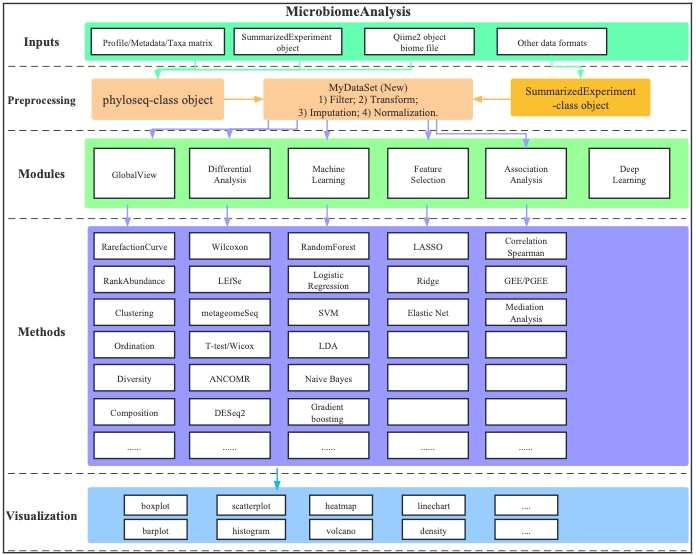
\includegraphics[width=1\linewidth,height=1\textheight]{./figures/Schematic} 

}

\caption{Flowchat of MicrobiomeAnalysis}\label{fig:unnamed-chunk-1}
\end{figure}

The data pre-processing module includes six main procedures:

\begin{itemize}
\tightlist
\item
  \textbf{Data Transformation}
\item
  \textbf{Data Imputation}
\item
  \textbf{Data Normalization}
\item
  \textbf{Data Scaling}
\item
  \textbf{Data Trimming}
\item
  \textbf{Data Filtering}
\end{itemize}

The downstream analysis includes several modules:

\begin{itemize}
\tightlist
\item
  \textbf{Diversity analysis}
\item
  \textbf{Ordination analysis}
\item
  \textbf{Clustering analysis}
\item
  \textbf{Differential analysis}
\item
  \textbf{Association analysis}
\end{itemize}

\hypertarget{input-data}{%
\section{Input data}\label{input-data}}

when using data pre-processing functions, it requires that the inputs which are from 16s or metagenomics data should be converted into phyloseq-class object:

\begin{itemize}
\item
  \textbf{Types of data}. Users can handle 16s or metagenomics data coming from any platform on a transformed phyloseq-class object when they use \texttt{import\_dada2} or \texttt{import\_qiime2}.
\item
  \textbf{Transformation}. The package provides multiple methods to transform individual values, such as log10,
\item
  \textbf{Imputation}. Missing value imputation methods also were provided by this package.
\item
  \textbf{Normalisation}. \texttt{MicrobiomeAnalysis} also has so many methods to normalize data sample by sample, which could remove technical effects.
\item
  \textbf{Prefiltering}. Removing low abundant taxa also could be done by using \texttt{MicrobiomeAnalysis}.
\item
  \textbf{Data format}. Most functions of \texttt{MicrobiomeAnalysis} are using phyloseq-class object as input. Therefore, users could convert their inputs into phyloseq-class object.
\end{itemize}

\hypertarget{methods}{%
\section{Methods}\label{methods}}

\hypertarget{some-background-knowledge}{%
\subsection{Some background knowledge}\label{some-background-knowledge}}

We list here the main methodological or theoretical concepts you need to know to be able to efficiently apply \texttt{MicrobiomeAnalysis}:

\begin{itemize}
\tightlist
\item
  \textbf{phyloseq-class, SummarizedExperiment-class}: the former object contains otu table, sample data and taxa table etc which are usually used in metagenomic data analysis. The latter one comprises expression data and metadata of gene, metabolites etc.
\end{itemize}

\hypertarget{key-publications}{%
\subsection{Key publications}\label{key-publications}}

\begin{itemize}
\item
  \textbf{phyloseq object}. \citep{mcmurdie2013phyloseq} phyloseq: an R package for reproducible interactive analysis and graphics of microbiome census data.
\item
  \textbf{Permutational Multivariate Analysis of Variance (PERMANOVA)}. \citep{anderson2014permutational} Permutational multivariate analysis of variance (PERMANOVA).
\item
  \textbf{ALDEx2}. \citep{fernandes2014unifying} Unifying the analysis of high-throughput sequencing datasets: characterizing RNA-seq, 16S rRNA gene sequencing and selective growth experiments by compositional data analysis.
\end{itemize}

\hypertarget{outline-of-this-tutorial}{%
\section{Outline of this tutorial}\label{outline-of-this-tutorial}}

\begin{itemize}
\item
  \textbf{Chapter \href{https://zouhua.top/MicrobiomeAnalysis_book/how-to-install-microbiomeanalysis.html}{2}}: How to install \texttt{MicrobiomeAnalysis}
\item
  \textbf{Chapter \href{https://zouhua.top/MicrobiomeAnalysis_book/data-processing.html}{3}}: Data Processing
\end{itemize}

\hypertarget{citation}{%
\section{Citation}\label{citation}}

Kindly cite by using citation(``MicrobiomeAnalysis'') if you think \texttt{MicrobiomeAnalysis} helps you. Alternative way is Zou H (2022). MicrobiomeAnalysis: An R package for analysis and visualization in metagenomics. R package version 1.0.3, \textless URL:\url{https://github.com/HuaZou/MicrobiomeAnalysis/}\textgreater.

\hypertarget{how-to-install-microbiomeanalysis}{%
\chapter{How to install MicrobiomeAnalysis}\label{how-to-install-microbiomeanalysis}}

Before installation, you should install the two following software.

\begin{itemize}
\item
  R 4.1.2 \citep{R-base} or later release \href{https://mirrors.tuna.tsinghua.edu.cn/CRAN/}{Download link}.
\item
  Rstudio Desktop \href{https://www.rstudio.com/products/rstudio/download/\#download}{Download link}.
\end{itemize}

\hypertarget{installation}{%
\section{Installation}\label{installation}}

First, installing either R package devtools or remotes:

\begin{Shaded}
\begin{Highlighting}[]
\ControlFlowTok{if}\NormalTok{ (}\SpecialCharTok{!}\FunctionTok{requireNamespace}\NormalTok{(}\FunctionTok{c}\NormalTok{(}\StringTok{"devtools"}\NormalTok{, }\StringTok{"remotes"}\NormalTok{), }\AttributeTok{quietly =} \ConstantTok{TRUE}\NormalTok{)) \{}
  \FunctionTok{install.packages}\NormalTok{(}\FunctionTok{c}\NormalTok{(}\StringTok{"devtools"}\NormalTok{, }\StringTok{"remotes"}\NormalTok{))}
\NormalTok{\}}

\NormalTok{devtools}\SpecialCharTok{::}\FunctionTok{install\_github}\NormalTok{(}\StringTok{"HuaZou/MicrobiomeAnalysis"}\NormalTok{)}
\CommentTok{\# remotes::install\_github("HuaZou/MicrobiomeAnalysis")}

\CommentTok{\# specific release}
\NormalTok{devtools}\SpecialCharTok{::}\FunctionTok{install\_github}\NormalTok{(}\StringTok{"HuaZou/MicrobiomeAnalysis@release{-}v1.0.3"}\NormalTok{)}
\end{Highlighting}
\end{Shaded}

Alternatively, you can install the latest released package from \href{https://github.com/HuaZou/MicrobiomeAnalysis/releases}{releases}:

\begin{Shaded}
\begin{Highlighting}[]
\FunctionTok{install.packages}\NormalTok{(}\StringTok{"MicrobiomeAnalysis*.tar.gz"}\NormalTok{, }\AttributeTok{repos =} \ConstantTok{NULL}\NormalTok{, }\AttributeTok{type =} \StringTok{"source"}\NormalTok{)}
\end{Highlighting}
\end{Shaded}

The \texttt{MicrobiomeAnalysis} package took \texttt{dplyr}, \texttt{phyloseq}, \texttt{purrr}, \texttt{magrittr}, \texttt{tibble}, \texttt{metagenomeSeq}, \texttt{biomformat}, \texttt{SummarizedExperiment}, \texttt{ggplot2} and \texttt{caret} etc as directly import packages.

\hypertarget{vignette}{%
\section{Vignette}\label{vignette}}

For brief introduction to use \texttt{MicrobiomeAnalysis}, please refer to vignette and choose \emph{html} format to do a practice.

\begin{Shaded}
\begin{Highlighting}[]
\NormalTok{utils}\SpecialCharTok{::}\FunctionTok{browseVignettes}\NormalTok{(}\AttributeTok{package=}\StringTok{"MicrobiomeAnalysis"}\NormalTok{)}
\end{Highlighting}
\end{Shaded}

\hypertarget{authors}{%
\section{Authors}\label{authors}}

\begin{itemize}
\tightlist
\item
  \href{mailto:zouhua1@outlook.com}{Hua Zou}
\end{itemize}

\hypertarget{data-processing}{%
\chapter{Data Processing}\label{data-processing}}

Outline of this Chapter:

\begin{itemize}
\item
  \protect\hyperlink{loading-packages}{Loading Packages}
\item
  \protect\hyperlink{importing-data}{Importing Data}
\item
  \protect\hyperlink{extracting-specific-levels}{Extracting specific levels}
\item
  \protect\hyperlink{summarizing-specific-levels}{Summarizing specific levels}
\item
  \protect\hyperlink{data-transformation}{Data Transformation}
\item
  \protect\hyperlink{data-imputation}{Data Imputation}
\item
  \protect\hyperlink{data-normalization}{Data Normalization}
\item
  \protect\hyperlink{data-scaling}{Data Scaling}
\item
  \protect\hyperlink{data-trimming}{Data Trimming}
\item
  \protect\hyperlink{data-filtering}{Data Filtering}
\end{itemize}

\hypertarget{loading-packages}{%
\section{Loading Packages}\label{loading-packages}}

\begin{Shaded}
\begin{Highlighting}[]
\FunctionTok{library}\NormalTok{(dplyr)}
\FunctionTok{library}\NormalTok{(tibble)}
\FunctionTok{library}\NormalTok{(phyloseq)}
\FunctionTok{library}\NormalTok{(SummarizedExperiment)}
\FunctionTok{library}\NormalTok{(MicrobiomeAnalysis)}
\end{Highlighting}
\end{Shaded}

\hypertarget{importing-data}{%
\section{Importing Data}\label{importing-data}}

\begin{itemize}
\tightlist
\item
  Converting the output of dada2 into phyloseq object
\end{itemize}

\begin{Shaded}
\begin{Highlighting}[]
\NormalTok{seq\_tab }\OtherTok{\textless{}{-}} \FunctionTok{readRDS}\NormalTok{(}
  \FunctionTok{system.file}\NormalTok{(}\StringTok{"extdata"}\NormalTok{, }\StringTok{"dada2\_seqtab.rds"}\NormalTok{,}
              \AttributeTok{package =} \StringTok{"MicrobiomeAnalysis"}\NormalTok{))}
\NormalTok{tax\_tab }\OtherTok{\textless{}{-}} \FunctionTok{readRDS}\NormalTok{(}
  \FunctionTok{system.file}\NormalTok{(}\StringTok{"extdata"}\NormalTok{, }\StringTok{"dada2\_taxtab.rds"}\NormalTok{,}
              \AttributeTok{package =} \StringTok{"MicrobiomeAnalysis"}\NormalTok{))}
\NormalTok{sam\_tab }\OtherTok{\textless{}{-}} \FunctionTok{read.table}\NormalTok{(}
  \FunctionTok{system.file}\NormalTok{(}\StringTok{"extdata"}\NormalTok{, }\StringTok{"dada2\_samdata.txt"}\NormalTok{,}
              \AttributeTok{package =} \StringTok{"MicrobiomeAnalysis"}\NormalTok{),}
  \AttributeTok{sep =} \StringTok{"}\SpecialCharTok{\textbackslash{}t}\StringTok{"}\NormalTok{, }\AttributeTok{header =} \ConstantTok{TRUE}\NormalTok{, }\AttributeTok{row.names =} \DecValTok{1}\NormalTok{)}

\NormalTok{ps\_dada2 }\OtherTok{\textless{}{-}} \FunctionTok{import\_dada2}\NormalTok{(}
   \AttributeTok{seq\_tab =}\NormalTok{ seq\_tab,}
   \AttributeTok{tax\_tab =}\NormalTok{ tax\_tab,}
   \AttributeTok{sam\_tab =}\NormalTok{ sam\_tab)}

\NormalTok{ps\_dada2}
\end{Highlighting}
\end{Shaded}

\begin{verbatim}
## phyloseq-class experiment-level object
## otu_table()   OTU Table:         [ 232 taxa and 20 samples ]
## sample_data() Sample Data:       [ 20 samples by 4 sample variables ]
## tax_table()   Taxonomy Table:    [ 232 taxa by 6 taxonomic ranks ]
## refseq()      DNAStringSet:      [ 232 reference sequences ]
\end{verbatim}

\begin{itemize}
\tightlist
\item
  Converting the qiime2 output of dada2 into phyloseq object
\end{itemize}

\begin{Shaded}
\begin{Highlighting}[]
\NormalTok{otuqza\_file }\OtherTok{\textless{}{-}} \FunctionTok{system.file}\NormalTok{(}
    \StringTok{"extdata"}\NormalTok{, }\StringTok{"table.qza"}\NormalTok{,}
    \AttributeTok{package =} \StringTok{"MicrobiomeAnalysis"}\NormalTok{)}
\NormalTok{taxaqza\_file }\OtherTok{\textless{}{-}} \FunctionTok{system.file}\NormalTok{(}
    \StringTok{"extdata"}\NormalTok{, }\StringTok{"taxonomy.qza"}\NormalTok{,}
    \AttributeTok{package =} \StringTok{"MicrobiomeAnalysis"}\NormalTok{)}
\NormalTok{sample\_file }\OtherTok{\textless{}{-}} \FunctionTok{system.file}\NormalTok{(}
    \StringTok{"extdata"}\NormalTok{, }\StringTok{"sample{-}metadata.tsv"}\NormalTok{,}
    \AttributeTok{package =} \StringTok{"MicrobiomeAnalysis"}\NormalTok{)}
\NormalTok{treeqza\_file }\OtherTok{\textless{}{-}} \FunctionTok{system.file}\NormalTok{(}
    \StringTok{"extdata"}\NormalTok{, }\StringTok{"tree.qza"}\NormalTok{,}
    \AttributeTok{package =} \StringTok{"MicrobiomeAnalysis"}\NormalTok{)}
\NormalTok{ps\_qiime2 }\OtherTok{\textless{}{-}} \FunctionTok{import\_qiime2}\NormalTok{(}
    \AttributeTok{otu\_qza =}\NormalTok{ otuqza\_file, }\AttributeTok{taxa\_qza =}\NormalTok{ taxaqza\_file,}
    \AttributeTok{sam\_tab =}\NormalTok{ sample\_file, }\AttributeTok{tree\_qza =}\NormalTok{ treeqza\_file}
\NormalTok{)}

\NormalTok{ps\_qiime2}
\end{Highlighting}
\end{Shaded}

\begin{verbatim}
## phyloseq-class experiment-level object
## otu_table()   OTU Table:         [ 770 taxa and 34 samples ]
## sample_data() Sample Data:       [ 34 samples by 9 sample variables ]
## tax_table()   Taxonomy Table:    [ 770 taxa by 7 taxonomic ranks ]
## phy_tree()    Phylogenetic Tree: [ 770 tips and 768 internal nodes ]
\end{verbatim}

\begin{itemize}
\tightlist
\item
  Convertings inputs into SummarizedExperiment object
\end{itemize}

\begin{Shaded}
\begin{Highlighting}[]
\FunctionTok{data}\NormalTok{(}\StringTok{"Zeybel\_2022\_protein"}\NormalTok{)}
\NormalTok{assay }\OtherTok{\textless{}{-}}\NormalTok{ SummarizedExperiment}\SpecialCharTok{::}\FunctionTok{assay}\NormalTok{(Zeybel\_2022\_protein) }\SpecialCharTok{\%\textgreater{}\%}
  \FunctionTok{data.frame}\NormalTok{()}
\NormalTok{rowData }\OtherTok{\textless{}{-}}\NormalTok{ SummarizedExperiment}\SpecialCharTok{::}\FunctionTok{rowData}\NormalTok{(Zeybel\_2022\_protein) }\SpecialCharTok{\%\textgreater{}\%}
  \FunctionTok{data.frame}\NormalTok{()}
\NormalTok{colData }\OtherTok{\textless{}{-}}\NormalTok{ SummarizedExperiment}\SpecialCharTok{::}\FunctionTok{colData}\NormalTok{(Zeybel\_2022\_protein) }\SpecialCharTok{\%\textgreater{}\%}
  \FunctionTok{data.frame}\NormalTok{()}
\NormalTok{metadata }\OtherTok{\textless{}{-}} \FunctionTok{list}\NormalTok{(}\AttributeTok{lab=}\StringTok{"hua"}\NormalTok{, }\AttributeTok{type=}\StringTok{"protein"}\NormalTok{)}

\NormalTok{assay }\OtherTok{\textless{}{-}}\NormalTok{ assay[}\DecValTok{1}\SpecialCharTok{:}\DecValTok{10}\NormalTok{, }\DecValTok{1}\SpecialCharTok{:}\DecValTok{10}\NormalTok{]}

\NormalTok{se\_protein }\OtherTok{\textless{}{-}} \FunctionTok{import\_SE}\NormalTok{(}
    \AttributeTok{object =}\NormalTok{ assay,}
    \AttributeTok{rowdata =}\NormalTok{ rowData,}
    \AttributeTok{coldata =}\NormalTok{ colData,}
    \AttributeTok{metadata =}\NormalTok{ metadata)}

\NormalTok{se\_protein}
\end{Highlighting}
\end{Shaded}

\begin{verbatim}
## class: SummarizedExperiment 
## dim: 10 10 
## metadata(2): lab type
## assays(1): ''
## rownames(10): IL8 VEGFA ... uPA IL6
## rowData names(3): ProteinID LOD prop
## colnames(10): P101001 P101003 ... P101013 P101016
## colData names(47): PatientID Gender ... Right_leg_fat_free_mass Right_leg_total_body_water
\end{verbatim}

\hypertarget{extracting-specific-levels}{%
\section{Extracting specific levels}\label{extracting-specific-levels}}

\begin{itemize}
\tightlist
\item
  Extracting ``Genus'' levels phyloseq object
\end{itemize}

\begin{Shaded}
\begin{Highlighting}[]
\NormalTok{ps\_genus }\OtherTok{\textless{}{-}} \FunctionTok{aggregate\_taxa}\NormalTok{(}\AttributeTok{x =}\NormalTok{ ps\_dada2, }
                           \AttributeTok{level =} \StringTok{"Genus"}\NormalTok{)}
\NormalTok{ps\_genus}
\end{Highlighting}
\end{Shaded}

\begin{verbatim}
## phyloseq-class experiment-level object
## otu_table()   OTU Table:         [ 66 taxa and 20 samples ]
## sample_data() Sample Data:       [ 20 samples by 4 sample variables ]
## tax_table()   Taxonomy Table:    [ 66 taxa by 7 taxonomic ranks ]
\end{verbatim}

\hypertarget{summarizing-specific-levels}{%
\section{Summarizing specific levels}\label{summarizing-specific-levels}}

\begin{itemize}
\tightlist
\item
  Phyloseq object contains from Kingdom to the the specific taxonomic levels (Phylum)
\end{itemize}

\begin{Shaded}
\begin{Highlighting}[]
\NormalTok{ps\_summarize\_genus }\OtherTok{\textless{}{-}} \FunctionTok{summarize\_taxa}\NormalTok{(}
    \AttributeTok{ps =}\NormalTok{ ps\_dada2, }
    \AttributeTok{level =} \StringTok{"Genus"}\NormalTok{)}
\NormalTok{ps\_summarize\_genus}
\end{Highlighting}
\end{Shaded}

\begin{verbatim}
## phyloseq-class experiment-level object
## otu_table()   OTU Table:         [ 66 taxa and 20 samples ]
## sample_data() Sample Data:       [ 20 samples by 4 sample variables ]
## tax_table()   Taxonomy Table:    [ 66 taxa by 1 taxonomic ranks ]
\end{verbatim}

\hypertarget{data-transformation}{%
\section{Data Transformation}\label{data-transformation}}

5 methods to transform individual values (\textbf{by individual value}).

\begin{itemize}
\item
  ``log10'', the transformation is log10(object), and if the data contains zeros the transformation is log10(1 + object).
\item
  ``log10p'', the transformation is log10(1 + object).
\item
  ``SquareRoot'', the transformation is Square Root.
\item
  ``CubicRoot'', the transformation is Cubic Root.
\item
  ``logit'', the transformation is Zero-inflated Logit Transformation (Does not work well for microbiome data).
\end{itemize}

Here is for \texttt{phyloseq-class}.

\begin{Shaded}
\begin{Highlighting}[]
\FunctionTok{data}\NormalTok{(}\StringTok{"Zeybel\_2022\_gut"}\NormalTok{)}
\NormalTok{ps\_transform }\OtherTok{\textless{}{-}} \FunctionTok{transform\_abundances}\NormalTok{(}
  \AttributeTok{object =}\NormalTok{ Zeybel\_2022\_gut,}
  \AttributeTok{level =} \StringTok{"Phylum"}\NormalTok{,}
  \AttributeTok{transform =} \StringTok{"log10p"}\NormalTok{)}

\FunctionTok{head}\NormalTok{(ps\_transform}\SpecialCharTok{@}\NormalTok{otu\_table}\SpecialCharTok{@}\NormalTok{.Data[, }\DecValTok{1}\SpecialCharTok{:}\DecValTok{5}\NormalTok{], }\DecValTok{3}\NormalTok{)}
\end{Highlighting}
\end{Shaded}

\begin{verbatim}
##                     P101003    P101007    P101010    P101012    P101018
## p__Actinobacteria -1.651096 -2.0986943 -2.5452009 -1.6773074 -1.8931057
## p__Bacteroidetes  -0.330115 -0.1437857 -0.3379679 -0.1574846 -0.1295813
## p__Chloroflexi     0.000000  0.0000000  0.0000000  0.0000000  0.0000000
\end{verbatim}

\begin{itemize}
\tightlist
\item
  Here is for \texttt{SummarizedExperiment-class}.
\end{itemize}

\begin{Shaded}
\begin{Highlighting}[]
\FunctionTok{data}\NormalTok{(}\StringTok{"Zeybel\_2022\_protein"}\NormalTok{)}
\NormalTok{se\_transform }\OtherTok{\textless{}{-}} \FunctionTok{transform\_abundances}\NormalTok{(}
  \AttributeTok{object =}\NormalTok{ Zeybel\_2022\_protein,}
  \AttributeTok{transform =} \StringTok{"SquareRoot"}\NormalTok{)}

\FunctionTok{head}\NormalTok{(}\FunctionTok{assay}\NormalTok{(se\_transform)[, }\DecValTok{1}\SpecialCharTok{:}\DecValTok{5}\NormalTok{], }\DecValTok{3}\NormalTok{)}
\end{Highlighting}
\end{Shaded}

\begin{verbatim}
##        P101001  P101003  P101004  P101007  P101009
## IL8   2.246691 2.063092 2.170020 2.400327 2.168238
## VEGFA 3.344589 3.302819 3.246115 3.321395 3.258289
## CD8A  3.398494 3.185073 3.132900 3.262700 3.075131
\end{verbatim}

\hypertarget{data-imputation}{%
\section{Data Imputation}\label{data-imputation}}

11 methods to impute missing value (NAs or Zeros)

\begin{itemize}
\item
  ``LOD'': specific Limit Of Detection which provides by user.
\item
  ``half\_min'': half minimal values across samples except zero.
\item
  ``median'': median values across samples except zero.
\item
  ``mean'': mean values across samples except zero.
\item
  ``min'': minimal values across samples except zero.
\item
  ``knn'': k-nearest neighbors samples.
\item
  ``rf'': nonparametric missing value imputation using Random Forest.
\item
  ``global\_mean'': a normal distribution with a mean that is down-shifted from the sample mean and a standard deviation that is a fraction of the standard deviation of the sample distribution.
\item
  ``svd'': missing values imputation based Singular value decomposition.
\item
  ``QRILC'': missing values imputation based quantile regression. (default: ``none'').
\end{itemize}

\texttt{phyloseq-class} as inputs

\begin{Shaded}
\begin{Highlighting}[]
\FunctionTok{data}\NormalTok{(}\StringTok{"Zeybel\_2022\_gut"}\NormalTok{)}
\NormalTok{ps\_impute }\OtherTok{\textless{}{-}} \FunctionTok{impute\_abundance}\NormalTok{(}
  \AttributeTok{object =}\NormalTok{ Zeybel\_2022\_gut,}
  \AttributeTok{level =} \StringTok{"Phylum"}\NormalTok{,}
  \AttributeTok{group =} \StringTok{"LiverFatClass"}\NormalTok{,}
  \AttributeTok{ZerosAsNA =} \ConstantTok{TRUE}\NormalTok{,}
  \AttributeTok{RemoveNA =} \ConstantTok{TRUE}\NormalTok{,}
  \AttributeTok{cutoff =} \DecValTok{20}\NormalTok{,}
  \AttributeTok{method =} \StringTok{"knn"}\NormalTok{)}

\FunctionTok{head}\NormalTok{(ps\_impute}\SpecialCharTok{@}\NormalTok{otu\_table}\SpecialCharTok{@}\NormalTok{.Data[, }\DecValTok{1}\SpecialCharTok{:}\DecValTok{5}\NormalTok{], }\DecValTok{3}\NormalTok{)}
\end{Highlighting}
\end{Shaded}

\begin{verbatim}
##                     P101003   P101007   P101010   P101012   P101018
## p__Actinobacteria 0.0223308 0.0079672 0.0028497 0.0210229 0.0127907
## p__Bacteroidetes  0.4676113 0.7181486 0.4592320 0.6958497 0.7420252
## p__Firmicutes     0.4818712 0.2715033 0.4577191 0.2712132 0.1701021
\end{verbatim}

\begin{itemize}
\tightlist
\item
  Inputs is from \texttt{SummarizedExperiment-class}.
\end{itemize}

\begin{Shaded}
\begin{Highlighting}[]
\FunctionTok{data}\NormalTok{(}\StringTok{"Zeybel\_2022\_protein"}\NormalTok{)}
\NormalTok{se\_impute }\OtherTok{\textless{}{-}} \FunctionTok{impute\_abundance}\NormalTok{(}
  \AttributeTok{object =}\NormalTok{ Zeybel\_2022\_protein,}
  \AttributeTok{group =} \StringTok{"LiverFatClass"}\NormalTok{,}
  \AttributeTok{ZerosAsNA =} \ConstantTok{TRUE}\NormalTok{,}
  \AttributeTok{RemoveNA =} \ConstantTok{TRUE}\NormalTok{,}
  \AttributeTok{cutoff =} \DecValTok{20}\NormalTok{,}
  \AttributeTok{method =} \StringTok{"knn"}\NormalTok{)}

\FunctionTok{head}\NormalTok{(}\FunctionTok{assay}\NormalTok{(se\_impute)[, }\DecValTok{1}\SpecialCharTok{:}\DecValTok{5}\NormalTok{], }\DecValTok{3}\NormalTok{)}
\end{Highlighting}
\end{Shaded}

\begin{verbatim}
##         P101001  P101003  P101004  P101007  P101009
## IL8    5.047325  4.25600  4.70867  5.76131  4.70094
## VEGFA 11.186140 10.90848 10.53712 11.03153 10.61631
## CD8A  11.549635 10.14454  9.81491 10.64507  9.45627
\end{verbatim}

\hypertarget{data-normalization}{%
\section{Data Normalization}\label{data-normalization}}

Normalizing the OTU\_table in phyloseq-class object sample by sample to reduce the effects of systematic differences such as library size (\textbf{by sample}).

\begin{itemize}
\item
  ``rarefy'': random subsampling counts to the smallest library size in the data set.
\item
  ``TSS'': total sum scaling, also referred to as ``relative abundance'', the abundances were normalized by dividing the corresponding sample library size.
\item
  ``TMM'': trimmed mean of m-values. First, a sample is chosen as reference. The scaling factor is then derived using a weighted trimmed mean over the differences of the log-transformed gene-count fold-change between the sample and the reference.
\item
  ``RLE'', relative log expression, RLE uses a pseudo-reference calculated using the geometric mean of the gene-specific abundances over all samples. The scaling factors are then calculated as the median of the gene counts ratios between the samples and the reference.
\item
  ``CSS'': cumulative sum scaling, calculates scaling factors as the cumulative sum of gene abundances up to a data-derived threshold.
\item
  ``CLR'': centered log-ratio normalization.
\item
  ``CPM'': pre-sample normalization of the sum of the values to 1e+06.
\end{itemize}

\begin{Shaded}
\begin{Highlighting}[]
\FunctionTok{data}\NormalTok{(}\StringTok{"caporaso"}\NormalTok{)}
\NormalTok{ps\_norm }\OtherTok{\textless{}{-}} \FunctionTok{normalize}\NormalTok{(}
    \AttributeTok{object =}\NormalTok{ caporaso,}
    \AttributeTok{method =} \StringTok{"TSS"}\NormalTok{)}

\FunctionTok{head}\NormalTok{(ps\_norm}\SpecialCharTok{@}\NormalTok{otu\_table}\SpecialCharTok{@}\NormalTok{.Data[, }\DecValTok{1}\SpecialCharTok{:}\DecValTok{5}\NormalTok{], }\DecValTok{3}\NormalTok{)}
\end{Highlighting}
\end{Shaded}

\begin{verbatim}
##                             L1S140       L1S208 L1S8 L1S281 L3S242
## New.CleanUp.ReferenceOTU647      0 0.0000000000    0      0      0
## 14030                            0 0.0000000000    0      0      0
## New.CleanUp.ReferenceOTU858      0 0.0001013993    0      0      0
\end{verbatim}

\hypertarget{data-scaling}{%
\section{Data Scaling}\label{data-scaling}}

Data scaling adjusts each variable/feature by a scaling factor computed based on the dispersion of the variable (\textbf{by variable/feature}).

\begin{itemize}
\item
  ``mean\_center'': values minus mean statistic.
\item
  ``zscore'': mean-centered and divided by the standard deviation of each variable.
\item
  ``pareto'': mean-centered and divided by the square root of the standard deviation of each variable.
\item
  ``range'': mean-centered and divided by the range of each variable. (default: ``none'').
\end{itemize}

\texttt{phyloseq-class} as inputs

\begin{Shaded}
\begin{Highlighting}[]
\FunctionTok{data}\NormalTok{(}\StringTok{"enterotypes\_arumugam"}\NormalTok{)}
\NormalTok{ps\_scale }\OtherTok{\textless{}{-}} \FunctionTok{scale\_variables}\NormalTok{(}
  \AttributeTok{object =}\NormalTok{ enterotypes\_arumugam,}
  \AttributeTok{level =} \StringTok{"Phylum"}\NormalTok{,}
  \AttributeTok{method =} \StringTok{"range"}\NormalTok{)}

\FunctionTok{head}\NormalTok{(ps\_scale}\SpecialCharTok{@}\NormalTok{otu\_table}\SpecialCharTok{@}\NormalTok{.Data[, }\DecValTok{1}\SpecialCharTok{:}\DecValTok{5}\NormalTok{], }\DecValTok{3}\NormalTok{)}
\end{Highlighting}
\end{Shaded}

\begin{verbatim}
##                    AM-AD-1     AM-AD-2  AM-F10-T1   AM-F10-T2    DA-AD-1
## Acidobacteria   0.00000000  0.00000000  0.0000000 0.000000000  0.0000000
## Actinobacteria  0.03379937 -0.05187261  0.0180014 0.882710081 -0.1132282
## Bacteroidetes  -0.21758868 -0.21769150 -0.0870175 0.004106405  0.4083952
\end{verbatim}

Inputs is from \texttt{SummarizedExperiment-class}.

\begin{Shaded}
\begin{Highlighting}[]
\FunctionTok{data}\NormalTok{(}\StringTok{"Zeybel\_2022\_protein"}\NormalTok{)}

\NormalTok{se\_impute }\OtherTok{\textless{}{-}} \FunctionTok{impute\_abundance}\NormalTok{(}
  \AttributeTok{object =}\NormalTok{ Zeybel\_2022\_protein,}
  \AttributeTok{group =} \StringTok{"LiverFatClass"}\NormalTok{,}
  \AttributeTok{ZerosAsNA =} \ConstantTok{TRUE}\NormalTok{,}
  \AttributeTok{RemoveNA =} \ConstantTok{TRUE}\NormalTok{,}
  \AttributeTok{cutoff =} \DecValTok{20}\NormalTok{,}
  \AttributeTok{method =} \StringTok{"knn"}\NormalTok{)}

\NormalTok{se\_scale }\OtherTok{\textless{}{-}} \FunctionTok{scale\_variables}\NormalTok{(}
\NormalTok{  se\_impute,}
  \AttributeTok{method =} \StringTok{"zscore"}\NormalTok{)}

\FunctionTok{head}\NormalTok{(}\FunctionTok{assay}\NormalTok{(se\_scale)[, }\DecValTok{1}\SpecialCharTok{:}\DecValTok{5}\NormalTok{], }\DecValTok{3}\NormalTok{)}
\end{Highlighting}
\end{Shaded}

\begin{verbatim}
##          P101001    P101003    P101004    P101007    P101009
## IL8   -0.6666419 -0.7058454 -0.5725945 -0.4119527 -0.5532427
## VEGFA  1.3465093  1.5156366  1.3859023  1.2384224  1.4615621
## CD8A   1.4657131  1.2605319  1.1432227  1.1174021  1.0664467
\end{verbatim}

\hypertarget{data-trimming}{%
\section{Data Trimming}\label{data-trimming}}

Trimming samples or features whose prevalence is less than threshold

\begin{itemize}
\item
  ``both'', prevalence of features and samples more than cutoff.
\item
  ``feature'', prevalence of features more than cutoff.
\item
  ``feature\_group'', prevalence of features more than cutoff by groups.
\item
  ``sample'', prevalence of samples more than cutoff.
\end{itemize}

\texttt{phyloseq-class} as inputs

\begin{Shaded}
\begin{Highlighting}[]
\FunctionTok{data}\NormalTok{(}\StringTok{"Zeybel\_2022\_gut"}\NormalTok{)}
\NormalTok{ps\_trim }\OtherTok{\textless{}{-}} \FunctionTok{trim\_prevalence}\NormalTok{(}
\NormalTok{  Zeybel\_2022\_gut,}
  \AttributeTok{group =} \StringTok{"LiverFatClass"}\NormalTok{,}
  \AttributeTok{level =} \StringTok{"Phylum"}\NormalTok{,}
  \AttributeTok{cutoff =} \FloatTok{0.1}\NormalTok{,}
  \AttributeTok{trim =} \StringTok{"feature\_group"}\NormalTok{)}

\NormalTok{ps\_trim}
\end{Highlighting}
\end{Shaded}

\begin{verbatim}
## phyloseq-class experiment-level object
## otu_table()   OTU Table:         [ 5 taxa and 42 samples ]
## sample_data() Sample Data:       [ 42 samples by 46 sample variables ]
## tax_table()   Taxonomy Table:    [ 5 taxa by 3 taxonomic ranks ]
\end{verbatim}

Inputs is from \texttt{SummarizedExperiment-class}.

\begin{Shaded}
\begin{Highlighting}[]
\FunctionTok{data}\NormalTok{(}\StringTok{"Zeybel\_2022\_protein"}\NormalTok{)}
\NormalTok{se\_trim }\OtherTok{\textless{}{-}} \FunctionTok{trim\_prevalence}\NormalTok{(}
\NormalTok{  Zeybel\_2022\_protein,}
  \AttributeTok{cutoff =} \FloatTok{0.99}\NormalTok{,}
  \AttributeTok{trim =} \StringTok{"both"}\NormalTok{)}
\NormalTok{se\_trim}
\end{Highlighting}
\end{Shaded}

\begin{verbatim}
## class: SummarizedExperiment 
## dim: 66 54 
## metadata(0):
## assays(1): ''
## rownames(66): IL8 VEGFA ... TNFB CSF_1
## rowData names(3): ProteinID LOD prop
## colnames(54): P101001 P101003 ... P101095 P101096
## colData names(47): PatientID Gender ... Right_leg_fat_free_mass Right_leg_total_body_water
\end{verbatim}

\hypertarget{data-filtering}{%
\section{Data Filtering}\label{data-filtering}}

Filtering feature who is low relative abundance or unclassified (Ref: \citep{thingholm2019obese})

\begin{itemize}
\item
  Feature is more than Mean relative abundance across all samples;
\item
  Feature is more than Minimum relative abundance at least one sample.
\end{itemize}

\texttt{phyloseq-class} as inputs

\begin{Shaded}
\begin{Highlighting}[]
\FunctionTok{data}\NormalTok{(}\StringTok{"Zeybel\_2022\_gut"}\NormalTok{)}
\NormalTok{Zeybel\_2022\_gut\_counts }\OtherTok{\textless{}{-}}\NormalTok{ phyloseq}\SpecialCharTok{::}\FunctionTok{transform\_sample\_counts}\NormalTok{(}
\NormalTok{Zeybel\_2022\_gut, }\ControlFlowTok{function}\NormalTok{(x) \{}\FunctionTok{round}\NormalTok{(x }\SpecialCharTok{*} \DecValTok{10}\SpecialCharTok{\^{}}\DecValTok{7}\NormalTok{)\})}

\CommentTok{\# absolute abundance}
\NormalTok{ps\_filter\_absolute }\OtherTok{\textless{}{-}} \FunctionTok{filter\_abundance}\NormalTok{(}
   \AttributeTok{object =}\NormalTok{ Zeybel\_2022\_gut\_counts,}
   \AttributeTok{level =} \StringTok{"Genus"}\NormalTok{,}
   \AttributeTok{cutoff\_mean =} \DecValTok{100}\NormalTok{,}
   \AttributeTok{cutoff\_one =} \DecValTok{1000}\NormalTok{,}
   \AttributeTok{unclass =} \ConstantTok{FALSE}\NormalTok{)}

\NormalTok{ps\_filter\_absolute}
\end{Highlighting}
\end{Shaded}

\begin{verbatim}
## phyloseq-class experiment-level object
## otu_table()   OTU Table:         [ 94 taxa and 42 samples ]
## sample_data() Sample Data:       [ 42 samples by 46 sample variables ]
## tax_table()   Taxonomy Table:    [ 94 taxa by 7 taxonomic ranks ]
\end{verbatim}

\begin{Shaded}
\begin{Highlighting}[]
\CommentTok{\# relative abundance}
\NormalTok{ps\_filter\_relative }\OtherTok{\textless{}{-}} \FunctionTok{filter\_abundance}\NormalTok{(}
   \AttributeTok{object =}\NormalTok{ Zeybel\_2022\_gut,}
   \AttributeTok{level =} \StringTok{"Genus"}\NormalTok{,}
   \AttributeTok{cutoff\_mean =} \FloatTok{1e{-}04}\NormalTok{,}
   \AttributeTok{cutoff\_one =} \FloatTok{1e{-}03}\NormalTok{,}
   \AttributeTok{unclass =} \ConstantTok{TRUE}\NormalTok{)}

\NormalTok{ps\_filter\_relative}
\end{Highlighting}
\end{Shaded}

\begin{verbatim}
## phyloseq-class experiment-level object
## otu_table()   OTU Table:         [ 67 taxa and 42 samples ]
## sample_data() Sample Data:       [ 42 samples by 46 sample variables ]
## tax_table()   Taxonomy Table:    [ 67 taxa by 7 taxonomic ranks ]
\end{verbatim}

Inputs is from \texttt{SummarizedExperiment-class}.

\begin{Shaded}
\begin{Highlighting}[]
\FunctionTok{data}\NormalTok{(}\StringTok{"Zeybel\_2022\_protein"}\NormalTok{)}
\NormalTok{se\_filter }\OtherTok{\textless{}{-}} \FunctionTok{filter\_abundance}\NormalTok{(}
  \AttributeTok{object =}\NormalTok{ Zeybel\_2022\_protein,}
  \AttributeTok{cutoff\_mean =} \DecValTok{5}\NormalTok{,}
  \AttributeTok{cutoff\_one =} \DecValTok{8}\NormalTok{)}

\NormalTok{se\_filter}
\end{Highlighting}
\end{Shaded}

\begin{verbatim}
## class: SummarizedExperiment 
## dim: 40 54 
## metadata(0):
## assays(1): ''
## rownames(40): 4E_BP1 AXIN1 ... uPA VEGFA
## rowData names(3): ProteinID LOD prop
## colnames(54): P101001 P101003 ... P101095 P101096
## colData names(47): PatientID Gender ... Right_leg_fat_free_mass Right_leg_total_body_water
\end{verbatim}

\hypertarget{systematic-information}{%
\section{Systematic Information}\label{systematic-information}}

\begin{Shaded}
\begin{Highlighting}[]
\NormalTok{devtools}\SpecialCharTok{::}\FunctionTok{session\_info}\NormalTok{()}
\end{Highlighting}
\end{Shaded}

\begin{verbatim}
## - Session info ---------------------------------------------------------------------------------------------------------------
##  setting  value
##  version  R version 4.1.2 (2021-11-01)
##  os       macOS Monterey 12.2.1
##  system   x86_64, darwin17.0
##  ui       RStudio
##  language (EN)
##  collate  en_US.UTF-8
##  ctype    en_US.UTF-8
##  tz       Asia/Shanghai
##  date     2023-01-12
##  rstudio  2022.07.2+576 Spotted Wakerobin (desktop)
##  pandoc   2.19.2 @ /Applications/RStudio.app/Contents/MacOS/quarto/bin/tools/ (via rmarkdown)
## 
## - Packages -------------------------------------------------------------------------------------------------------------------
##  package              * version  date (UTC) lib source
##  ade4                   1.7-18   2021-09-16 [1] CRAN (R 4.1.0)
##  ANCOMBC                1.4.0    2021-10-26 [1] Bioconductor
##  annotate               1.72.0   2021-10-26 [1] Bioconductor
##  AnnotationDbi          1.56.2   2021-11-09 [1] Bioconductor
##  ape                    5.6-2    2022-03-02 [1] CRAN (R 4.1.2)
##  assertthat             0.2.1    2019-03-21 [1] CRAN (R 4.1.0)
##  Biobase              * 2.54.0   2021-10-26 [1] Bioconductor
##  BiocGenerics         * 0.40.0   2021-10-26 [1] Bioconductor
##  BiocParallel           1.28.3   2021-12-09 [1] Bioconductor
##  biomformat             1.22.0   2021-10-26 [1] Bioconductor
##  Biostrings             2.62.0   2021-10-26 [1] Bioconductor
##  bit                    4.0.4    2020-08-04 [1] CRAN (R 4.1.0)
##  bit64                  4.0.5    2020-08-30 [1] CRAN (R 4.1.0)
##  bitops                 1.0-7    2021-04-24 [1] CRAN (R 4.1.0)
##  blob                   1.2.2    2021-07-23 [1] CRAN (R 4.1.0)
##  bookdown               0.29     2022-09-12 [1] CRAN (R 4.1.2)
##  brio                   1.1.3    2021-11-30 [1] CRAN (R 4.1.0)
##  bslib                  0.4.0    2022-07-16 [1] CRAN (R 4.1.2)
##  cachem                 1.0.6    2021-08-19 [1] CRAN (R 4.1.0)
##  callr                  3.7.0    2021-04-20 [1] CRAN (R 4.1.0)
##  caTools                1.18.2   2021-03-28 [1] CRAN (R 4.1.0)
##  cli                    3.4.1    2022-09-23 [1] CRAN (R 4.1.2)
##  cluster                2.1.2    2021-04-17 [1] CRAN (R 4.1.2)
##  codetools              0.2-18   2020-11-04 [1] CRAN (R 4.1.2)
##  colorspace             2.0-3    2022-02-21 [1] CRAN (R 4.1.2)
##  crayon                 1.5.0    2022-02-14 [1] CRAN (R 4.1.2)
##  data.table             1.14.6   2022-11-16 [1] CRAN (R 4.1.2)
##  DBI                    1.1.2    2021-12-20 [1] CRAN (R 4.1.0)
##  DelayedArray           0.20.0   2021-10-26 [1] Bioconductor
##  desc                   1.4.1    2022-03-06 [1] CRAN (R 4.1.2)
##  DESeq2                 1.34.0   2021-10-26 [1] Bioconductor
##  devtools               2.4.3    2021-11-30 [1] CRAN (R 4.1.0)
##  digest                 0.6.30   2022-10-18 [1] CRAN (R 4.1.2)
##  dplyr                * 1.0.10   2022-09-01 [1] CRAN (R 4.1.2)
##  ellipsis               0.3.2    2021-04-29 [1] CRAN (R 4.1.0)
##  evaluate               0.17     2022-10-07 [1] CRAN (R 4.1.2)
##  fansi                  1.0.2    2022-01-14 [1] CRAN (R 4.1.2)
##  fastmap                1.1.0    2021-01-25 [1] CRAN (R 4.1.0)
##  foreach                1.5.2    2022-02-02 [1] CRAN (R 4.1.2)
##  fs                     1.5.2    2021-12-08 [1] CRAN (R 4.1.0)
##  genefilter             1.76.0   2021-10-26 [1] Bioconductor
##  geneplotter            1.72.0   2021-10-26 [1] Bioconductor
##  generics               0.1.2    2022-01-31 [1] CRAN (R 4.1.2)
##  GenomeInfoDb         * 1.30.1   2022-01-30 [1] Bioconductor
##  GenomeInfoDbData       1.2.7    2022-03-09 [1] Bioconductor
##  GenomicRanges        * 1.46.1   2021-11-18 [1] Bioconductor
##  ggplot2                3.4.0    2022-11-04 [1] CRAN (R 4.1.2)
##  glmnet                 4.1-3    2021-11-02 [1] CRAN (R 4.1.0)
##  glue                   1.6.2    2022-02-24 [1] CRAN (R 4.1.2)
##  gplots                 3.1.1    2020-11-28 [1] CRAN (R 4.1.0)
##  gtable                 0.3.0    2019-03-25 [1] CRAN (R 4.1.0)
##  gtools                 3.9.2    2021-06-06 [1] CRAN (R 4.1.0)
##  highr                  0.9      2021-04-16 [1] CRAN (R 4.1.0)
##  htmltools              0.5.3    2022-07-18 [1] CRAN (R 4.1.2)
##  httr                   1.4.2    2020-07-20 [1] CRAN (R 4.1.0)
##  igraph                 1.2.11   2022-01-04 [1] CRAN (R 4.1.2)
##  impute                 1.68.0   2021-10-26 [1] Bioconductor
##  IRanges              * 2.28.0   2021-10-26 [1] Bioconductor
##  iterators              1.0.14   2022-02-05 [1] CRAN (R 4.1.2)
##  jquerylib              0.1.4    2021-04-26 [1] CRAN (R 4.1.0)
##  jsonlite               1.8.3    2022-10-21 [1] CRAN (R 4.1.2)
##  KEGGREST               1.34.0   2021-10-26 [1] Bioconductor
##  KernSmooth             2.23-20  2021-05-03 [1] CRAN (R 4.1.2)
##  knitr                  1.40     2022-08-24 [1] CRAN (R 4.1.2)
##  lattice                0.20-45  2021-09-22 [1] CRAN (R 4.1.2)
##  lifecycle              1.0.3    2022-10-07 [1] CRAN (R 4.1.2)
##  limma                  3.50.1   2022-02-17 [1] Bioconductor
##  locfit                 1.5-9.5  2022-03-03 [1] CRAN (R 4.1.2)
##  magrittr               2.0.3    2022-03-30 [1] CRAN (R 4.1.2)
##  MASS                   7.3-55   2022-01-13 [1] CRAN (R 4.1.2)
##  Matrix                 1.4-0    2021-12-08 [1] CRAN (R 4.1.0)
##  MatrixGenerics       * 1.6.0    2021-10-26 [1] Bioconductor
##  matrixStats          * 0.61.0   2021-09-17 [1] CRAN (R 4.1.0)
##  memoise                2.0.1    2021-11-26 [1] CRAN (R 4.1.0)
##  metagenomeSeq          1.36.0   2021-10-26 [1] Bioconductor
##  mgcv                   1.8-39   2022-02-24 [1] CRAN (R 4.1.2)
##  microbiome             1.16.0   2021-10-26 [1] Bioconductor
##  MicrobiomeAnalysis   * 1.0.3    2023-01-12 [1] Bioconductor
##  multtest               2.50.0   2021-10-26 [1] Bioconductor
##  munsell                0.5.0    2018-06-12 [1] CRAN (R 4.1.0)
##  nlme                   3.1-155  2022-01-13 [1] CRAN (R 4.1.2)
##  nloptr                 2.0.0    2022-01-26 [1] CRAN (R 4.1.2)
##  permute                0.9-7    2022-01-27 [1] CRAN (R 4.1.2)
##  phyloseq             * 1.38.0   2021-10-26 [1] Bioconductor
##  pillar                 1.7.0    2022-02-01 [1] CRAN (R 4.1.2)
##  pkgbuild               1.3.1    2021-12-20 [1] CRAN (R 4.1.0)
##  pkgconfig              2.0.3    2019-09-22 [1] CRAN (R 4.1.0)
##  pkgload                1.2.4    2021-11-30 [1] CRAN (R 4.1.0)
##  plyr                   1.8.6    2020-03-03 [1] CRAN (R 4.1.0)
##  png                    0.1-7    2013-12-03 [1] CRAN (R 4.1.0)
##  prettyunits            1.1.1    2020-01-24 [1] CRAN (R 4.1.0)
##  processx               3.5.2    2021-04-30 [1] CRAN (R 4.1.0)
##  ps                     1.6.0    2021-02-28 [1] CRAN (R 4.1.0)
##  purrr                  0.3.4    2020-04-17 [1] CRAN (R 4.1.0)
##  R6                     2.5.1    2021-08-19 [1] CRAN (R 4.1.0)
##  rbibutils              2.2.7    2021-12-07 [1] CRAN (R 4.1.0)
##  RColorBrewer           1.1-2    2014-12-07 [1] CRAN (R 4.1.0)
##  Rcpp                   1.0.9    2022-07-08 [1] CRAN (R 4.1.2)
##  RCurl                  1.98-1.6 2022-02-08 [1] CRAN (R 4.1.2)
##  Rdpack                 2.2      2022-03-19 [1] CRAN (R 4.1.2)
##  remotes                2.4.2    2021-11-30 [1] CRAN (R 4.1.0)
##  reshape2               1.4.4    2020-04-09 [1] CRAN (R 4.1.0)
##  rhdf5                  2.38.1   2022-03-10 [1] Bioconductor
##  rhdf5filters           1.6.0    2021-10-26 [1] Bioconductor
##  Rhdf5lib               1.16.0   2021-10-26 [1] Bioconductor
##  rlang                  1.0.6    2022-09-24 [1] CRAN (R 4.1.2)
##  rmarkdown              2.17     2022-10-07 [1] CRAN (R 4.1.2)
##  rprojroot              2.0.2    2020-11-15 [1] CRAN (R 4.1.0)
##  RSQLite                2.2.10   2022-02-17 [1] CRAN (R 4.1.2)
##  rstudioapi             0.13     2020-11-12 [1] CRAN (R 4.1.0)
##  Rtsne                  0.15     2018-11-10 [1] CRAN (R 4.1.0)
##  S4Vectors            * 0.32.3   2021-11-21 [1] Bioconductor
##  sass                   0.4.2    2022-07-16 [1] CRAN (R 4.1.2)
##  scales                 1.2.1    2022-08-20 [1] CRAN (R 4.1.2)
##  sessioninfo            1.2.2    2021-12-06 [1] CRAN (R 4.1.0)
##  shape                  1.4.6    2021-05-19 [1] CRAN (R 4.1.0)
##  stringi                1.7.8    2022-07-11 [1] CRAN (R 4.1.2)
##  stringr                1.4.1    2022-08-20 [1] CRAN (R 4.1.2)
##  SummarizedExperiment * 1.24.0   2021-10-26 [1] Bioconductor
##  survival               3.4-0    2022-08-09 [1] CRAN (R 4.1.2)
##  testthat               3.1.2    2022-01-20 [1] CRAN (R 4.1.2)
##  tibble               * 3.1.8    2022-07-22 [1] CRAN (R 4.1.2)
##  tidyr                  1.2.0    2022-02-01 [1] CRAN (R 4.1.2)
##  tidyselect             1.1.2    2022-02-21 [1] CRAN (R 4.1.2)
##  usethis                2.1.5    2021-12-09 [1] CRAN (R 4.1.0)
##  utf8                   1.2.2    2021-07-24 [1] CRAN (R 4.1.0)
##  vctrs                  0.5.1    2022-11-16 [1] CRAN (R 4.1.2)
##  vegan                  2.5-7    2020-11-28 [1] CRAN (R 4.1.0)
##  withr                  2.5.0    2022-03-03 [1] CRAN (R 4.1.2)
##  Wrench                 1.12.0   2021-10-26 [1] Bioconductor
##  xfun                   0.34     2022-10-18 [1] CRAN (R 4.1.2)
##  XML                    3.99-0.9 2022-02-24 [1] CRAN (R 4.1.2)
##  xtable                 1.8-4    2019-04-21 [1] CRAN (R 4.1.0)
##  XVector                0.34.0   2021-10-26 [1] Bioconductor
##  yaml                   2.3.6    2022-10-18 [1] CRAN (R 4.1.2)
##  zlibbioc               1.40.0   2021-10-26 [1] Bioconductor
## 
##  [1] /Library/Frameworks/R.framework/Versions/4.1/Resources/library
## 
## ------------------------------------------------------------------------------------------------------------------------------
\end{verbatim}

  \bibliography{assets/book.bib,assets/packages.bib}

\end{document}
